\documentclass[12pt,a4paper,twoside]{article}
\usepackage{labor}
\begin{document}

%fill for cover and header creation
\newcommand\laboratorynumber{2}
\title{Gitter/Prisma}
\newcommand\supervisor{Weis, Valentin}
\newcommand\groupnumber{42}

\newcommand\participantonelastname{Eisner}
\newcommand\participantonefirstname{Nico}
\newcommand\participantoneid{12214121}
\newcommand\participanttwolastname{Waldl}
\newcommand\participanttwofirstname{Philip}
\newcommand\participanttwoid{12214120}
\author{\participantonelastname \ \& \participanttwolastname}

\newcommand\degreeid{UB 033 678}
\newcommand\semester{23WS}
\date{13.10.2023}

%select correct course title
%\newcommand\coursetitle{Einführung in die \\ physikalischen Messmethoden}
%\newcommand\coursetitle{Laborübungen 1: \\ Mechanik und Wärme}
\newcommand\coursetitle{Laborübungen 2: \\ Elektrizität, Magnetismus, Optik}
%\newcommand\coursetitle{Fortgeschrittenen Praktikum 1: \\ Technische Physik}
%\newcommand\coursetitle{Fortgeschrittenen Praktikum 2: \\ Allgemeine Physik}

%\begin{titlepage}
   \begin{center}
       \begin{figure}[H]
            \begin{minipage}[h]{30mm}
                \centerline{
\includegraphics[height=15mm]{cover_nudes/tugraz.png}}
            \end{minipage}
            \hfill
            \begin{minipage}[h]{30mm}
                \centerline{
\includegraphics[height=15mm]{cover_nudes/nawi_graz.png}}
            \end{minipage}
            \hfill
            \begin{minipage}[h]{30mm}
                \centerline{
\includegraphics[height=15mm]{cover_nudes/uni-graz.png}}
            \end{minipage}
        \end{figure}
        
        \large{\emph{Institut für Experimentalphysik der Technischen Universität Graz \\
        \& Institut für Physik der Universität Graz}} \\
        \vspace{5mm}
        
        {\Huge \textbf{\coursetitle}}
        \vspace{5mm}
        
        {\huge \laboratorynumber: \thetitle}
    \end{center}
    
    \vfill
    
    \begin{table}[H]
        \LARGE
        \centering
        \begin{tabular}{r l}
            Betreuer:       & \supervisor \\
            Gruppennummer:  & \groupnumber \\
            \\
            Name:           & \participantonelastname, \participantonefirstname \\
            Matrikelnummer: & \participantoneid \\
            Name:           & \participanttwolastname, \participanttwofirstname \\
            Matrikelnummer: & \participanttwoid \\
            \\
            Kennzahl:       & \degreeid \\
            Datum:          & \semester \ | \thedate
        \end{tabular}
    \end{table}
    \vspace{4cm}
\end{titlepage}
\clearpage
\setcounter{page}{1}

%\maketitle %short title alternative

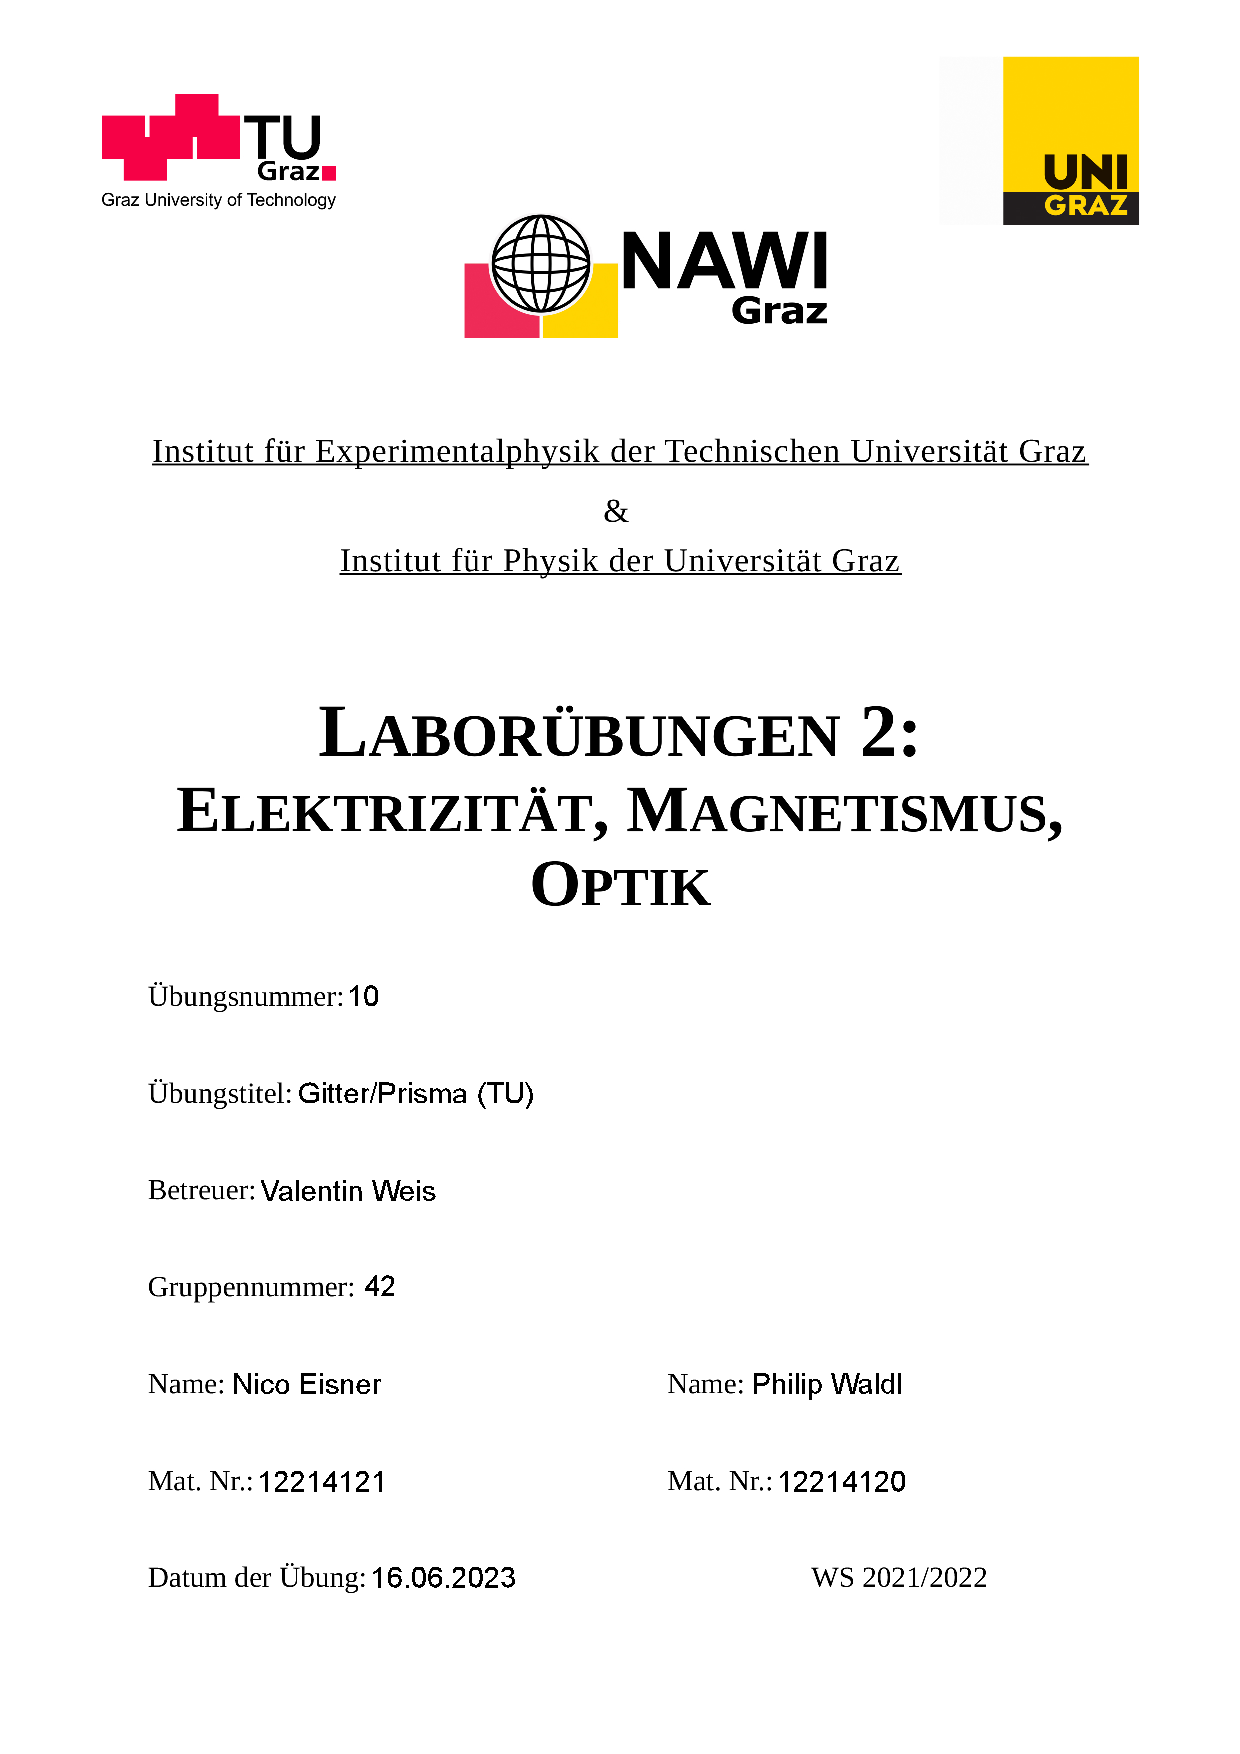
\includepdf[pages={1}]{../Deckblätter/Deckblatt_Gitter.pdf}

\tableofcontents
\newpage

\section{Aufgabenstellung} %jo beschreibn wos gmocht host ------------------------------
Das Experiment Gitter/Prisma ist in zwei Teile gegliedert. Die Aufgabe beim Gitter ist es, die Gitterkonstante $g$ mithilfe einer gelben Na-Dampflampe zu bestimmen, sowie die Wellenlänge $\lambda$ der sichtbaren Linien einer Spektrallampe. 
\\
Im zweiten Teil des Experimentes besteht die Aufgabe den brechenden Winkel eines Prismas $\gamma$ durch Messung des Reflexionswinkels $\epsilon$ zu bestimmen. 
Des weiteren ist auch der Brechungsindex $n(\lambda_0)$ des Prismas für die gut sichtbaren Linien einer Hg-Dampflampe zu bestimmen. 
\\
\\
Alle Informationen und Methodiken wurden uns von der Technischen Universität bereitgestellt \cite{teachcenter2}. 

\section{Voraussetzungen \& Grundlagen} %Grundlagen erklären, Formeln mit erklärung
\subsection{Gitter}
Ein Gitter besteht aus lichtdurchlässigen Öffnungen und lichtblockenden Balken, welche in bestimmten Abständen folgen. Ein gutes Beispiel für ein Gitter ist eine Jalousie. 
In diesem Fall besteht das Gitter aus einer Glasplatte. Fällt Licht auf dieses Gitter, wird es gebeugt und von jeden Punkt einer Öffnung gehen Kugelförmige Lichtwellen aus, welche sich nach Richtung und Wellenlänge durch Interferenzen verstärken oder abschwächen. 
\\
\\
%Bild
\\
Durch viele aufeinanderfolgende Balken in regelmäßigen Öffnungsabständen $g$ (Gitterkonstante) können alle neuen Wellen interferieren. Dabei tritt je nach Winkel $\varphi$ eine konstruktive oder destruktive Interferenz auf. 
Die konstruktiven Interferenzen können als Beugungsmaxima der Wellenlänge $\lambda$ beobachtet werden. 

    \begin{equation}
        \label{eq:Gitterkonstante}
        \centerline{$\Delta=g sin(\varphi) = z\lambda$,     $z \in \mathbb{Z} $}
    \end{equation}

\noindent
Die Zahl $z$ ist die Ordnungszahl des Beugungsmaximums. 

\subsection{Prisma}
Licht wird durch einen Prisma gebrochen. 
Die Bahn eines einfarbigen Lichtstrahls einer Frequenz durch verschiedene Medien wird eindeutig festgelegt. Die entscheidenden Faktoren sind dabei die Brechungsindizes der verschiedenen Medien, die geometrische Form und Lage ihrer Begrenzungsflächen. 
Reflektionen und Brechungen treten an der Grenze zweier Medien mit verschiedenen Brechungsindizes auf. Der Einfallende Strahl $E$ wird im selben Winkel $\alpha$ mit dem Lot $L$ wieder Reflektiert $R$. 
Der Winkel $\beta$ zwischen gebrochenen Strahl $G$ und Lot $L$ wird mithilfe des Brechungsgesetzes von Snellius berechnet. 

\begin{equation}
    \label{eq:Snellius}
    \centerline{$sin(\alpha) n_1 = sin(\beta) n_2$}
\end{equation}

\begin{figure}[H]
    \centering
    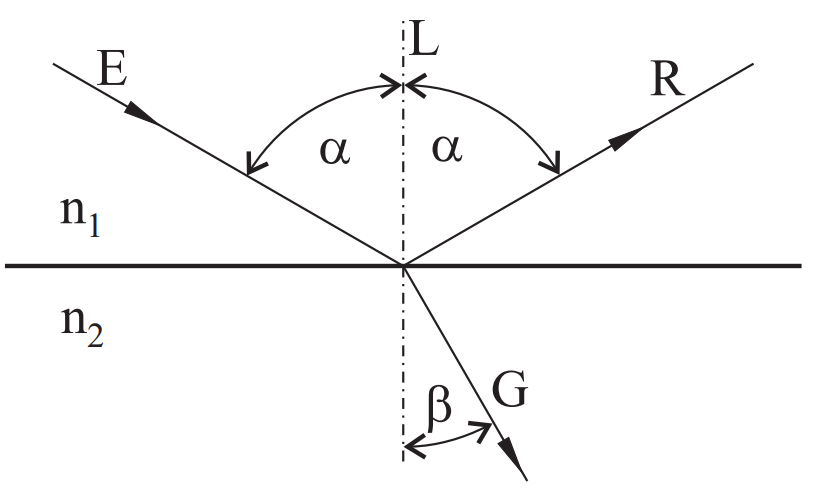
\includegraphics[width=0.6\linewidth]{nudes/Brechung.png}
    \caption{Brechung und Reflexion an einen Übergang. \cite{teachcenter2}}
    \label{fig:brechung}
\end{figure}

\noindent
Bei einen Strahlengang durch den Prisma wird das Licht zwei mal gebrochen. 
Das Licht ändert seine Richtung unter dem Ablenkungswinkel $\delta $ bei einem symmetrischen Strahlengang. Hierbei ist der Ein- und Austrittswinkel gleich groß. 
Dieser Winkel kann durch schwenken des Prismas leicht gefunden werden. 
Misst man nun den Winkel $\omega$ zwischen zwei zum einfallenden Strahl symmetrischen Lagen des Prismas, kann der Ablenkungswinkel $\delta $ berechnet werden. 

\begin{equation}
    \label{eq:Ablenkungswinkel}
    \centerline{$\delta = \omega /2$}
\end{equation}

\noindent
Formt man nun die Gleichung auf den Brechungsindex $n$ des Prismas um, so erhält man

\begin{equation}
    \label{eq:Brechungsindex}
    \centerline{$ n = \frac{sin(\frac{\gamma + \delta }{2})}{sin(\gamma /2)}$}
\end{equation}
dies lässt sich jedoch nur bei symmetrischen Strahlengang bewerkstelligen. 

\section{Versuchsanordnung} %mit skizze kurz beschreiben ------------------------------
Der Aufbau des Versuches mit dem Gitter ist wiefolgt. Es besteht aus einen Spektrometertisch. Dieser ist in Kollimator, einen Fernrohr auf einer rotierbaren Winkelskala und einer Ablage für Gitter und Prisma in der Mitte. 
Die Lichtquellen sind eine Quecksilberlampe und eine Natriumlampe, welche je nach Versuch an die Öffnung des Kollimators gestellt. 
Durch die in den Kollimator verbaute Schlitzblende wird die Stärke bzw. Helligkeit des Lichtstrahles eingestellt. 
Das Licht, welches durch den Kollimator parallelisiert wird, trifft auf das Gitter, im späteren Verlauf auf den Prisma, und wird dort gebrochen/gebeugt. 
Mit dem Fernrohr lässt sich das Licht nun beobachten und durch das Fadenkreuz kann ein einzelner Strahl genauestens anvisiert werden. 

    \begin{figure}[H]
        \centering
        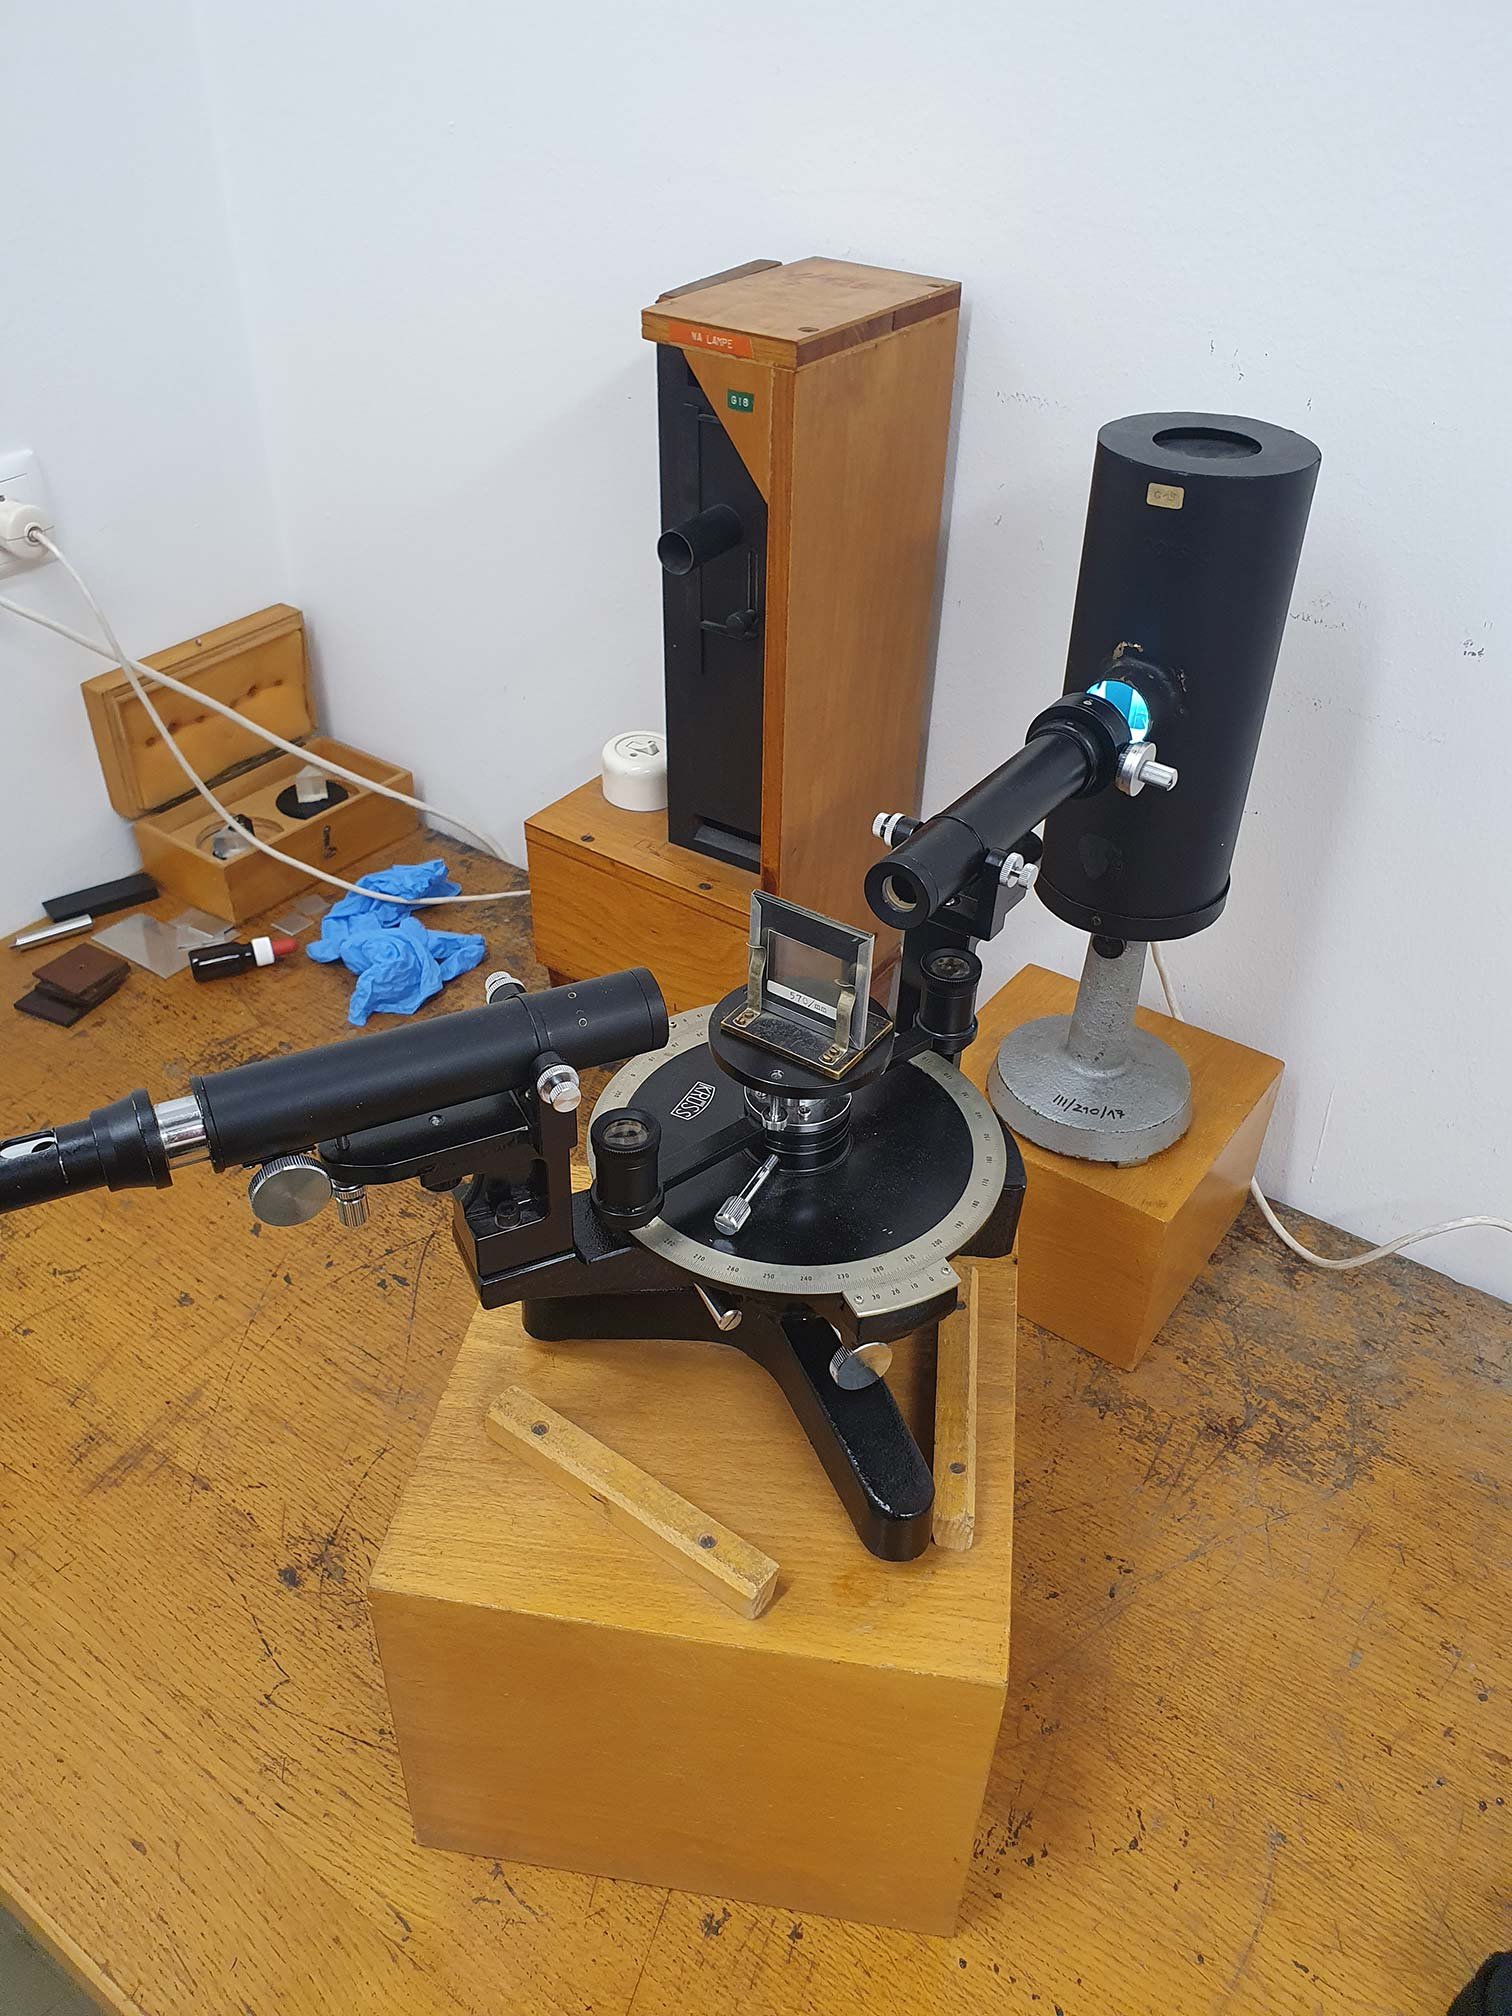
\includegraphics[width=0.6\linewidth, angle=-90]{nudes/versuch.jpg}
        \caption{Aufbau des Spektrometertisches}
        \label{fig:Aufbau}
    \end{figure}
\noindent
Das Fernrohr wird für die Messung des Winkels nach links und rechts gescwenkt und auf der Winkelskala der entsprechende Winkel abgelesen. 

\begin{figure}[H]
    \centering
    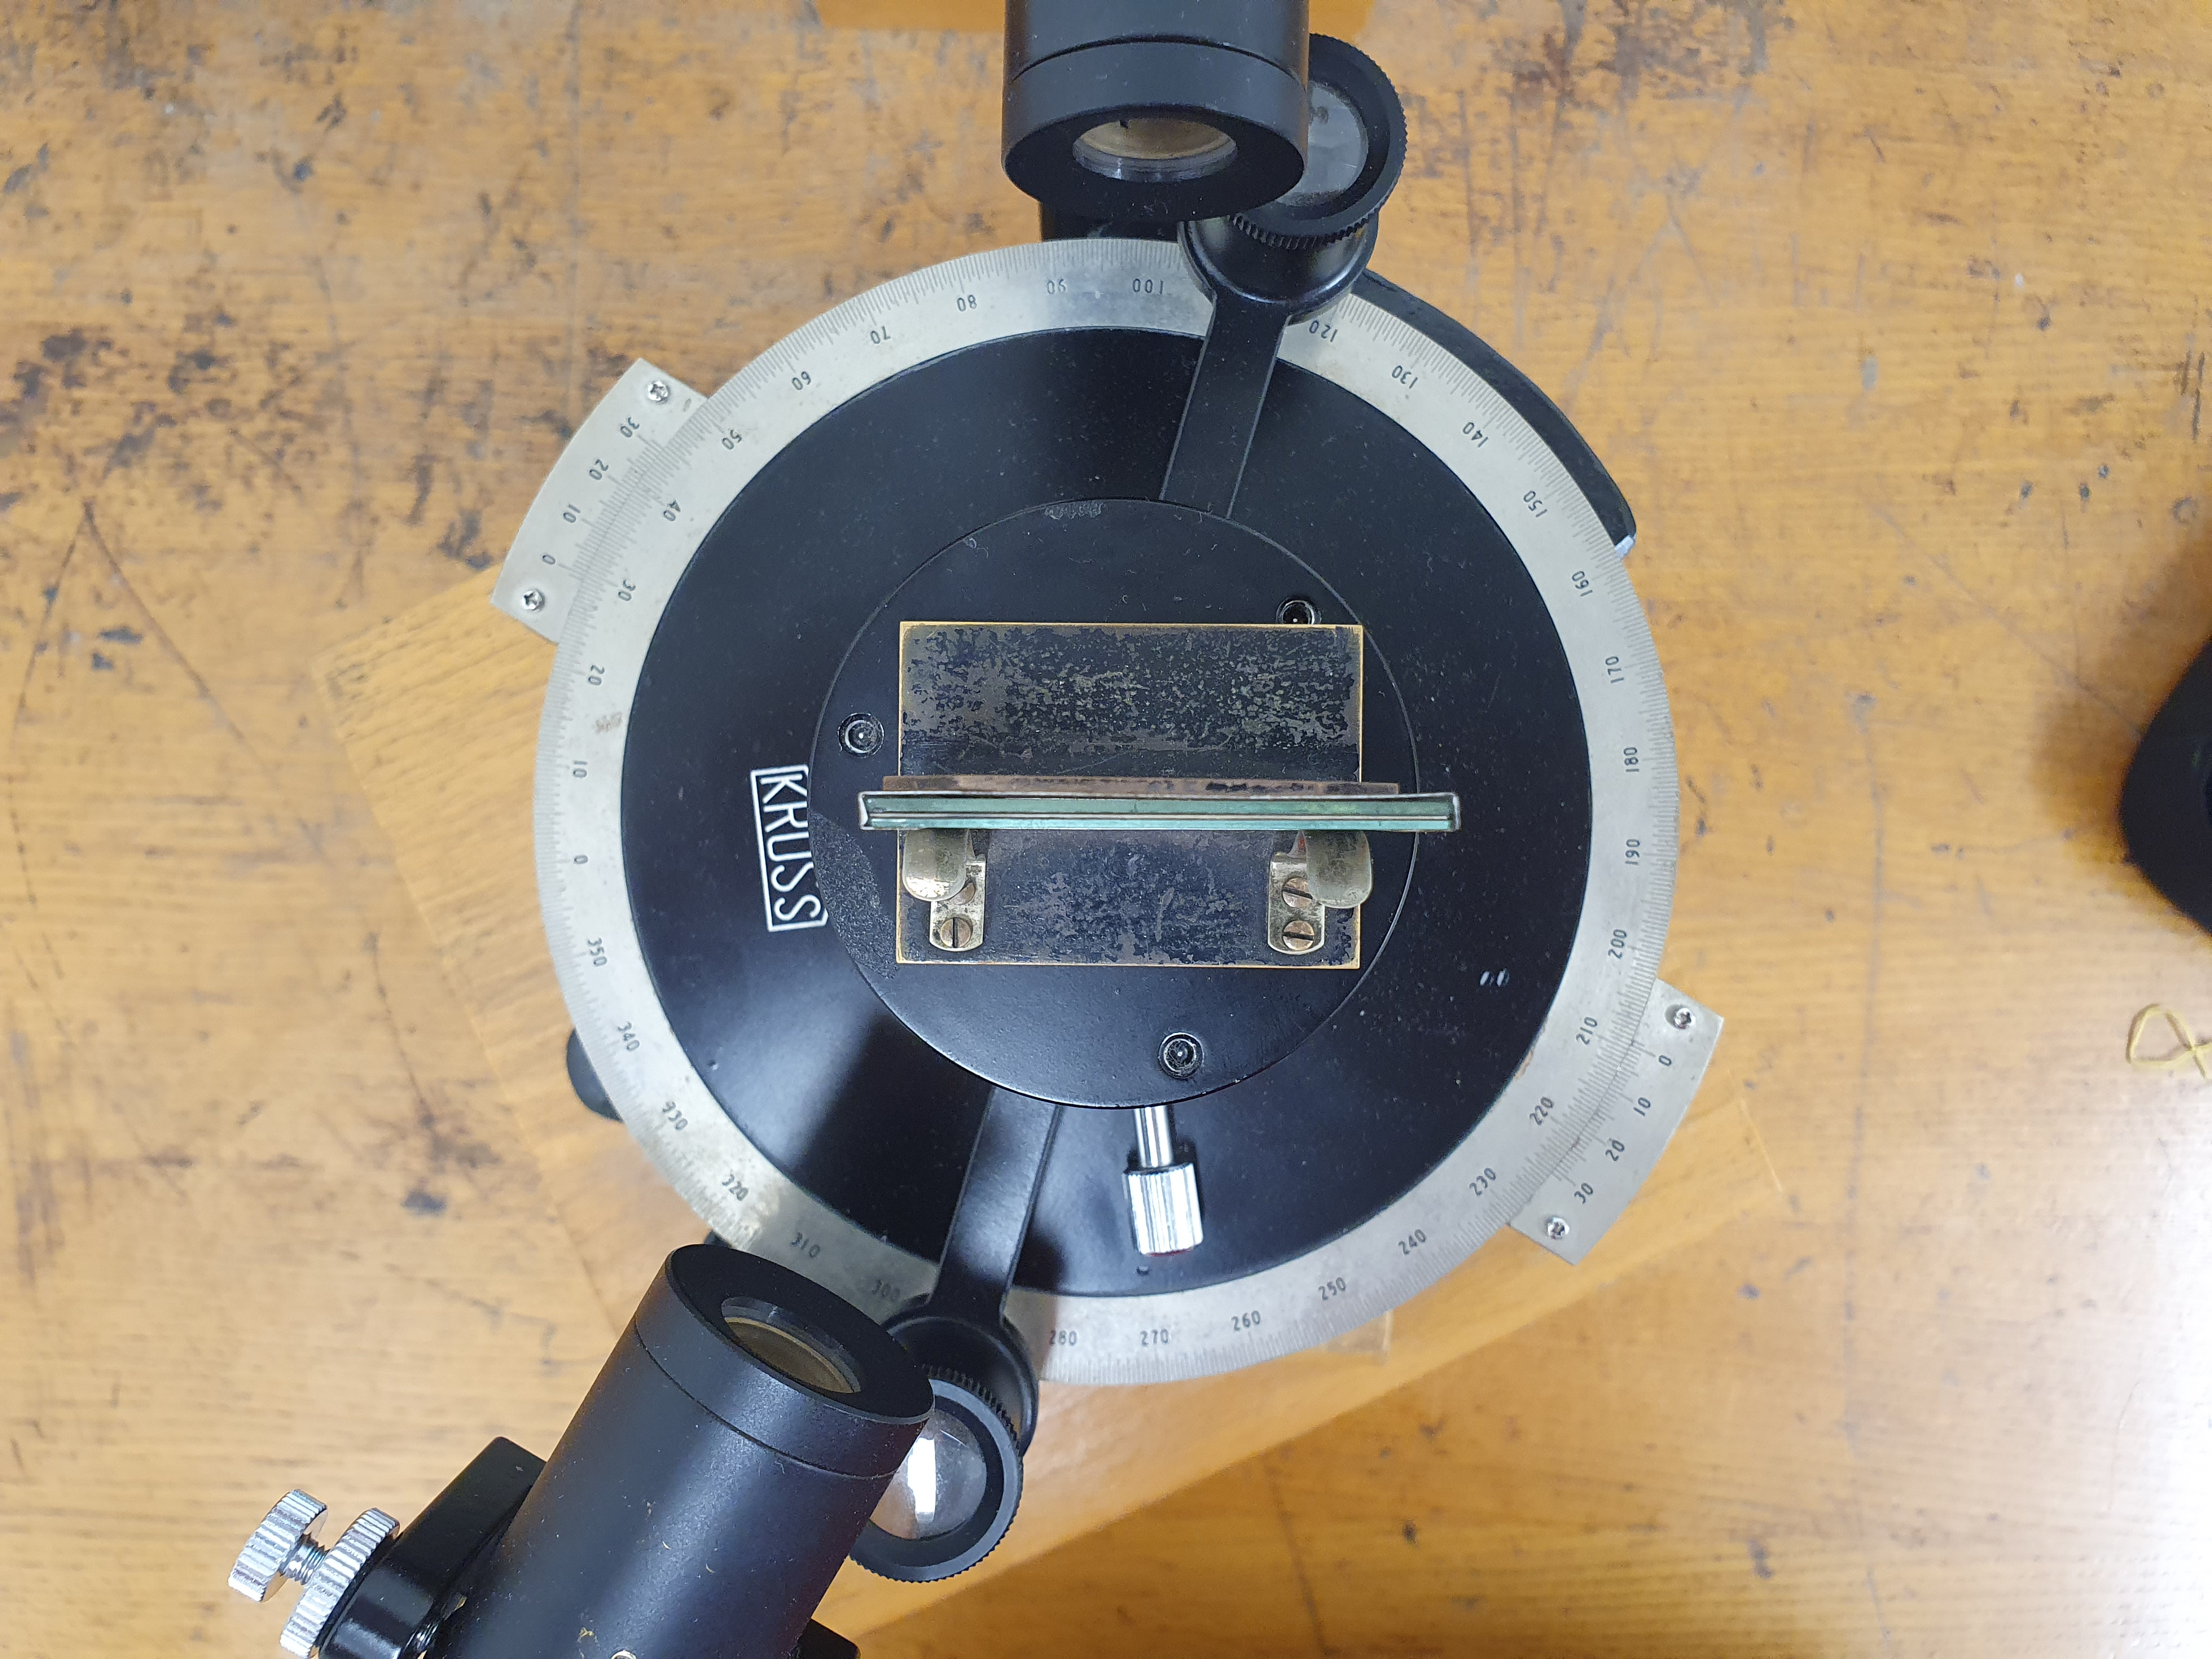
\includegraphics[width=0.6\linewidth, angle=-90]{nudes/messskala.jpg}
    \caption{Winkelskala}
    \label{fig:Winkelskala}
\end{figure}

\begin{figure}[H]
    \centering
    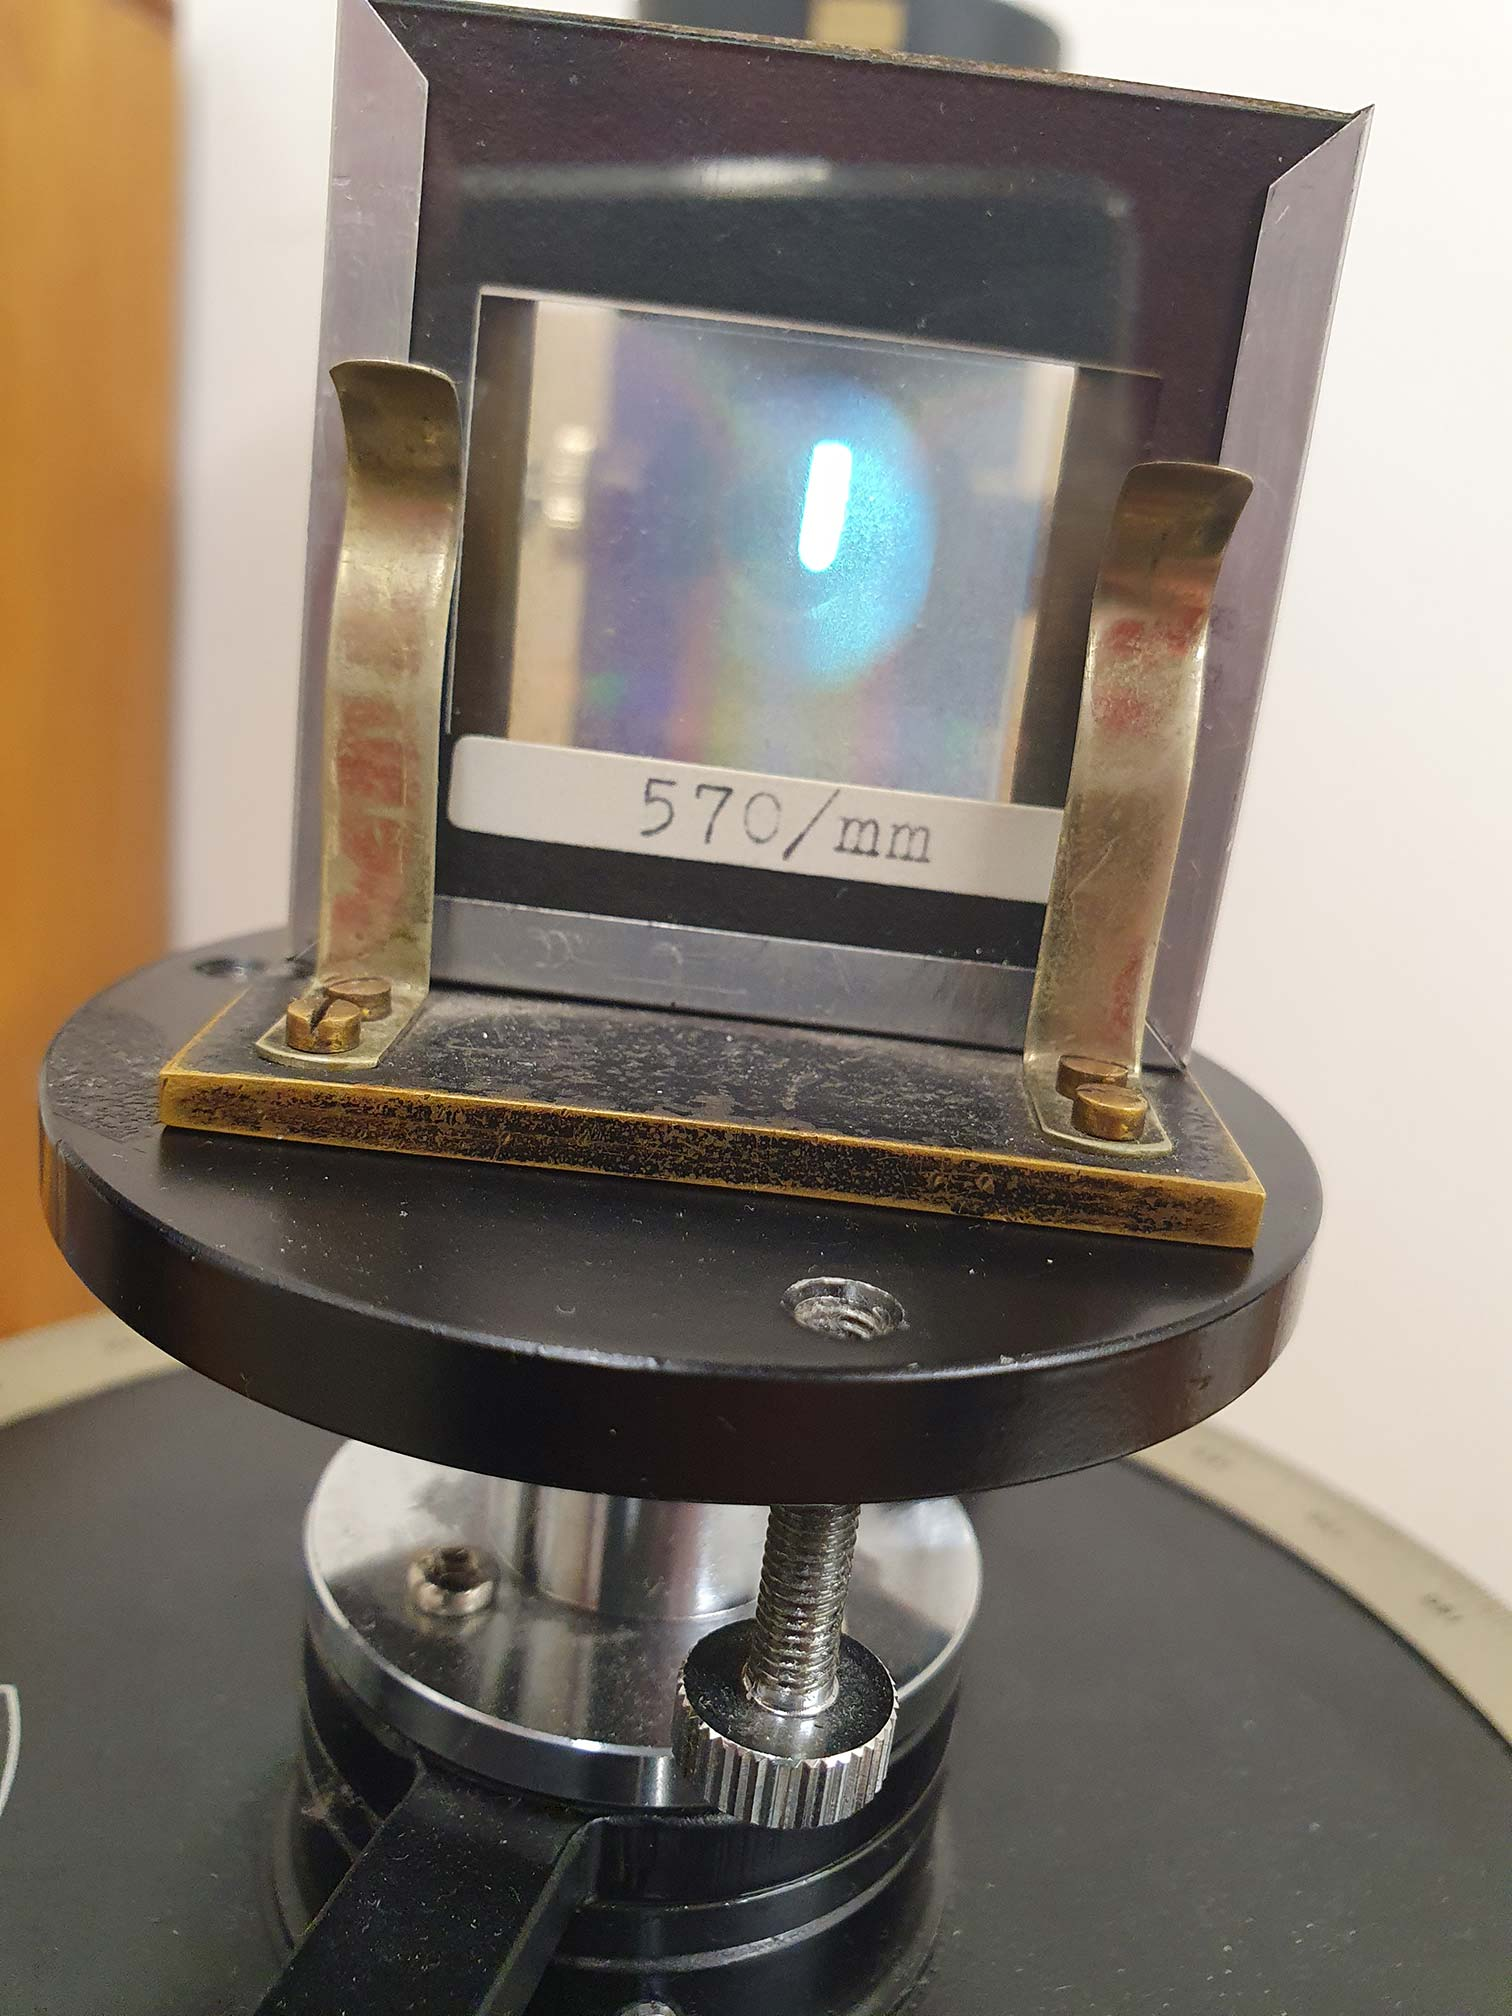
\includegraphics[width=0.6\linewidth, angle=-90]{nudes/gitter.jpg}
    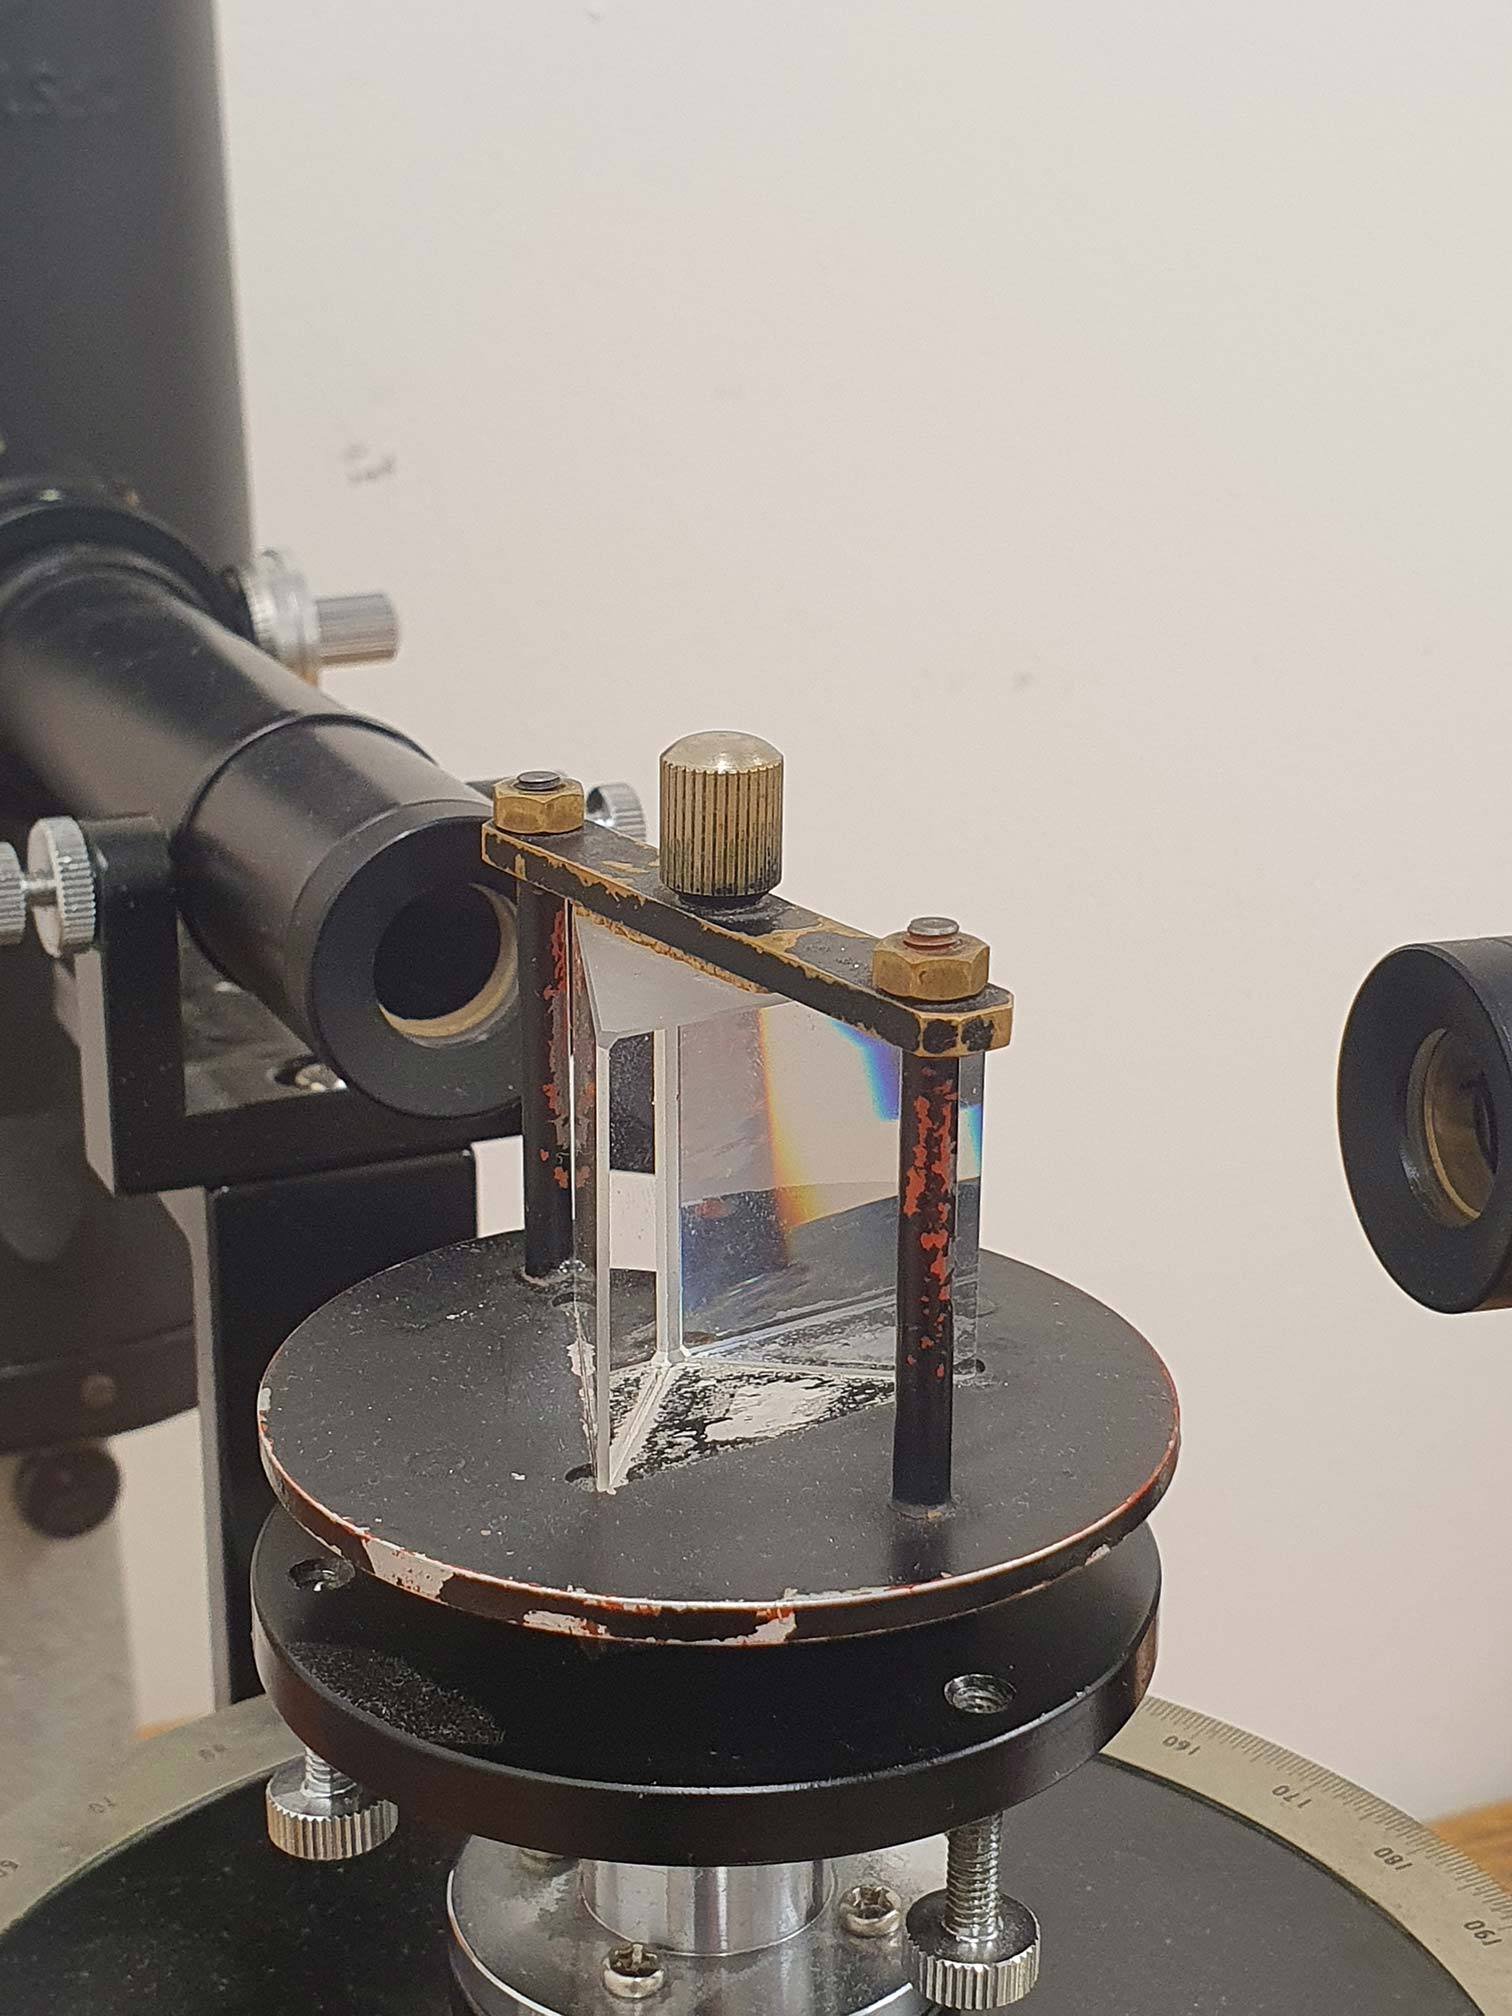
\includegraphics[width=0.6\linewidth, angle=-90]{nudes/prisma.jpg}
    \caption{Gitter (links) und Prisma (rechts)}
    \label{fig:gitterundprisma}
\end{figure}    


\section{Geräteliste} %jo holt a listn ------------------------------

    \begin{table}[H]
        \centering
        \caption{Im Versuch verwendete Geräte und Utensilien.}
        \label{tab:geraete}
        \begin{tabular}{| l | l | l |}
            \hline
            Gerät  & Gerätenummer  & Unsicherheit \\
            \hline
            Quecksilberlampe & {n.a} & {n.a} \\
            Natriumlampe & G18 & {n.a} \\
            Gitter 570/mm & {n.a} & {n.a} \\
            Prisma & {n.a} & {n.a} \\
            Spektrometertisch & 0161165 & {n.a} \\
            Winkelskala & {n.a} & 1 bogenminute \\
            \hline
        \end{tabular}
    \end{table}


\section{Versuchsdurchführung \& Messergebnisse} %nachvollziehbar und klar dargestellt ------------------------------
Die Versuchsdurchführung besteht aus mehreren Teilen für das Gitter und Prisma. 
Der erste Teil besteht darin das Gitter zu Justieren. Dies war bereits der Fall und es wurde nur noch überprüft, dass keine Fehler vorhanden sind. Das Gitter wird mittig und normal zum Kollimator gestellt, wie in Bild \ref{fig:Aufbau} der Versuchsanordnung zu erkennen ist. 
Die Natriumlampe wird vor den Kollimator gestellt und die Blende so eingestellt, dass eine dünne, jedoch noch gut sichtbare Linie durch das Fernrohr zu erkennen ist. 
Durch schwenken des Fernrohres wird kontrolliert, ob zwei Maxima der Spektrallinien pro Seite sichtbar sind. 


\begin{table}[H]
    \centering
    \caption{Natriumlampe Gitter}
    \label{tab:Gitter v1}
    \begin{tabular}{| l | l | l |}
        \hline
        Nr.  & Links  & Rechts \\
        \hline
        1 & 41 + (2 $\pm$ 1) & 140 + (0 $\pm$ 1) \\
        2 & 41 + (1 $\pm$ 1) & 139 + (5 $\pm$ 1) \\
        3 & 41 + (5 $\pm$ 1) & 139 + (5 $\pm$ 1) \\
        4 & 41 + (4 $\pm$ 1) & 139 + (4 $\pm$ 1) \\
        5 & 41 + (1 $\pm$ 1) & 139 + (5 $\pm$ 1) \\
        \hline
    \end{tabular}
\end{table}

\begin{table}[H]
    \centering
    \caption{Quecksilberlampe Gitter}
    \label{tab:Gitter v2}
    \begin{tabular}{| l | l | l | l |}
        \hline
        Farbe & Nr. & Links  & Rechts \\
        \hline
        \hline
                &  1 & 48 + (4 $\pm$ 1) & 132 + (21 $\pm$ 1) \\
        rot     &  2 & 48 + (4 $\pm$ 1) & 132 + (20 $\pm$ 1) \\
                &  3 & 48 + (5 $\pm$ 1) & 132 + (20 $\pm$ 1) \\
        \hline
                &  1 & 41 + (17 $\pm$ 1) & 138 + (26 $\pm$ 1) \\
        gelb    &  2 & 41 + (17 $\pm$ 1) & 138 + (26 $\pm$ 1) \\
                &  3 & 41 + (17 $\pm$ 1) & 138 + (26 $\pm$ 1) \\
        \hline
                &  1 & 36 + (0 $\pm$ 1) & 144 + (7 $\pm$ 1) \\
        grün    &  2 & 36 + (0 $\pm$ 1) & 144 + (7 $\pm$ 1) \\
                &  3 & 36 + (1 $\pm$ 1) & 144 + (8 $\pm$ 1) \\
        \hline
                &  1 & 33 + (10 $\pm$ 1) & 146 + (20 $\pm$ 1) \\
        hellblau&  2 & 33 + (10 $\pm$ 1) & 146 + (20 $\pm$ 1) \\
                &  3 & 33 + (11 $\pm$ 1) & 146 + (20 $\pm$ 1) \\
        \hline
                &  1 & 27 + (24 $\pm$ 1) & 155 + (5 $\pm$ 1) \\
        lila    &  2 & 27 + (25 $\pm$ 1) & 152 + (5 $\pm$ 1) \\
                &  3 & 27 + (25 $\pm$ 1) & 152 + (5 $\pm$ 1) \\
        \hline
    \end{tabular}
\end{table}


\begin{table}[H]
    \centering
    \caption{Prisma}
    \label{tab:Prisma}
    \begin{tabular}{| l | l | l |}
        \hline
        Nr.  & Links  & Rechts \\
        \hline
        1 & 70 +    (4 $\pm$ 1) & 129 + (23 $\pm$ 1) \\
        2 & 69.5 +  (6 $\pm$ 1) & 129 + (23 $\pm$ 1) \\
        3 & 70 +    (4 $\pm$ 1) & 129 + (21 $\pm$ 1) \\
        4 & 70 +    (4 $\pm$ 1) & 129 + (22 $\pm$ 1) \\
        5 & 69.5 +  (4 $\pm$ 1) & 128 + (23 $\pm$ 1) \\
        6 & 70 +    (4 $\pm$ 1) & 129 + (22 $\pm$ 1) \\
        \hline
    \end{tabular}
\end{table}


\begin{table}[H]
    \centering
    \caption{Quecksilberlampe Gitter}
    \label{tab:Prisma v2}
    \begin{tabular}{| l | l | l | l |}
        \hline
        Farbe & Nr. & Links  & Rechts \\
        \hline
        \hline
                &  1 & 38 + (6 $\pm$ 1) & 97.5 + (17 $\pm$ 1) \\
        rot     &  2 & 38 + (5 $\pm$ 1) & 97.5 + (17 $\pm$ 1) \\
                &  3 & 38 + (6 $\pm$ 1) & 97.5 + (17 $\pm$ 1) \\
        \hline
                &  1 & 38.5 + (0 $\pm$ 1) & 98 + (10 $\pm$ 1) \\
        gelb    &  2 & 38.5 + (1 $\pm$ 1) & 98 + (10 $\pm$ 1) \\
                &  3 & 38.5 + (0 $\pm$ 1) & 98 + (11 $\pm$ 1) \\
        \hline
                &  1 & 38.5 + (13 $\pm$ 1) & 98 + (24 $\pm$ 1) \\
        grün    &  2 & 38.5 + (13 $\pm$ 1) & 98 + (25 $\pm$ 1) \\
                &  3 & 38.5 + (13 $\pm$ 1) & 98 + (24 $\pm$ 1) \\
        \hline
                &  1 & 39 + (0 $\pm$ 1) & 98.5 + (5 $\pm$ 1) \\
        hellblau&  2 & 39 + (0 $\pm$ 1) & 98.5 + (6 $\pm$ 1) \\
                &  3 & 39 + (1 $\pm$ 1) & 98.5 + (6 $\pm$ 1) \\
        \hline
                &  1 & 39.5 + (6 $\pm$ 1) & 98.5 + (23 $\pm$ 1) \\
        lila    &  2 & 39.5 + (6 $\pm$ 1) & 98.5 + (22 $\pm$ 1) \\
                &  3 & 39.5 + (6 $\pm$ 1) & 98.5 + (23 $\pm$ 1) \\
        \hline
    \end{tabular}
\end{table}

\section{Auswertung und Unsicherheitsanalyse} %Nicht nur zahlen angeben ------------------------------

In der Auswertung werden zur erhöhten Genauigkeit durchgehend ungerundete Werte bis zu den Endergebnissen verwendet und nur zur Darstellung gerundet. \\
Zur Berechnung der Unsicherheiten wird, wenn nicht anders angegeben, die Größtunsicherheitsmethode verwendet.


\section{Diskussion} %diskussion der Unsicherheiten und Ergebnisse und evtl. verlgeich mit Literatur ------------------------------


\section{Zusammenfassung} %klare, übersichtliche vollständige beantwortung der Aufgabenstellung ------------------------------


\printbibliography[heading=bibintoc]
\end{document}
